\documentclass[a4paper,10pt,twocolumn,english]{article}
%---------------------------------------------------------
\usepackage{babel}
\usepackage[utf8]{inputenc}
\usepackage[T1]{fontenc}
\usepackage{hyperref}
\usepackage{graphicx}
\usepackage[ruled,vlined,linesnumbered]{algorithm2e}
\usepackage{bm}
\usepackage{listings}
\usepackage{xcolor}

\definecolor{codegreen}{rgb}{0,0.6,0}
\definecolor{codegray}{rgb}{0.5,0.5,0.5}
\definecolor{codepurple}{rgb}{0.58,0,0.82}
\definecolor{backcolour}{rgb}{0.95,0.95,0.92}

\lstdefinestyle{mystyle}
{
    backgroundcolor=\color{backcolour},   
    commentstyle=\color{codegreen},
    keywordstyle=\color{magenta},
    numberstyle=\tiny\color{codegray},
    stringstyle=\color{codepurple},
    basicstyle=\ttfamily\footnotesize,
    breakatwhitespace=false,         
    breaklines=true,                 
    captionpos=b,                    
    keepspaces=true,                 
    numbers=left,                    
    numbersep=5pt,                  
    showspaces=false,                
    showstringspaces=false,
    showtabs=false,                  
    tabsize=2
}

\lstset{style=mystyle}

\graphicspath{ {./images/} }

%---------------------------------------------------------

\title{Remote Timing Attacks: Exposing RSA Private Keys}

\author{
    Ioan Ionescu, 
    Radu Tomescu,
    Virgil Turcu\\
	\footnotesize Computer Science Department, University of Bucharest, Romania
}

\date{\empty} % no need for a date

\begin{document}
\maketitle
%---------------------------------------------------------
\begin{abstract} 
% Write here one or two paragraphs about what you will treat in the current paper:
% topic,
% methods,
% solutions,
% comparison results etc.
\end{abstract}
%---------------------------------------------------------
\section{Introduction}

% In this section you introduce the problem and existing research or similar results in the field.

% When citing remember you can use the quotes button from \url{https://scholar.google.com} to get the bibtex entry.

% In this article we are going to investigate side-channel attacks~\cite{kocher96_timing}
% with focus on cache implementations~\cite{lipp18_meltdown}.

%---------------------------------------------------------
\section{Technical description of the problem}

% In this section you describe the technical details of the articles you surveyed.



%---------------------------------------------------------
\section{Possible solution}


%---------------------------------------------------------
\section{Experiments and Results}
The experiments conducted in the paper aim to clarify the proper requirements
for the attack to work and to test the overall efficiency of the attack in various environments.

The first experiment, which is the most relevant, is split into two sections: the first one is to illustrate that increasing
the sample size for each bit guessing attempt provides a better chance to expose the private key;
the second one aims to prove that the size of the neighborhood over which we query each guess is directly proportional to the zero-one bit gap. 

The first part is quite intuitive. Its result shows, in simple terms, how trying to guess a bit of the $q$ multiple times will yield a higher chance of actually guessing that bit right. 
This is a direct consequence of the Law of Large Numbers, which states that the sample mean tends to the expected value of the distribution that models a trial as the sample size approaches infinity.

\begin{figure}[ht]
    \centering
    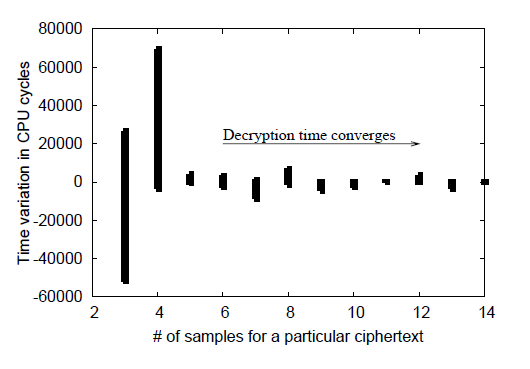
\includegraphics[width=0.9\linewidth]{ExperimentVariance.png}
    \caption{Variance evolution as sample size increases}
    \label{fig:experiment1a}
\end{figure}


The second part of the experiment is based on the measurement $T_g$ defined in the previous section
and shows how increasing the neighborhood over which we query increases the difference in decryption time that
indicates whether the current bit of $q$ is 1 or 0. This is, without a doubt, the most relevant conclusion of this article, 
because it provides a solution to bypass "Sliding window multiplication".

To further solidify this outcome we provide our own simulation of this experiment, realized in R.
The following statements are our statistical assumptions:

\begin{itemize}
    \item $DecryptTime(g)$ can be modelled by an exponential random variable $Exp(\lambda)$ where $\lambda=1/ExpectedDecryptionTime$.
    \item Increasing the $g+i$ sequence translates to increasing the sample size for the exponential random variable.
    \item All trials over a neighborhood are independent.
\end{itemize}

Having taken into consideration the previous assumptions, and the result that states that the sum of identical and independent exponential random variables is a $\Gamma$ distribution, we obtain the following:

\[T_g=\left(\sum_{i=0}^{n} DecryptTime(g+i)\right) \sim \Gamma(n,\lambda)\] 

\lstinputlisting[language=R, caption={R simulation code}, label={lst:simulation}]{code/experiment.R}

In Listing ~\ref*{lst:simulation} we have the R code used for generating the plot in Figure ~\ref*{fig:experiment1b_simulated}.

\begin{figure}[ht]
    \centering
    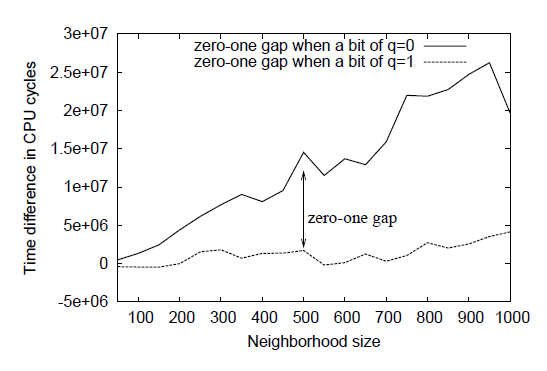
\includegraphics[width=0.9\linewidth]{ExpermimentArticol.png}
    \caption{Measured Evolution of $T_g$ difference}
    \label{fig:experiment1b_measured}
\end{figure}

\begin{figure}[ht]
    \centering
    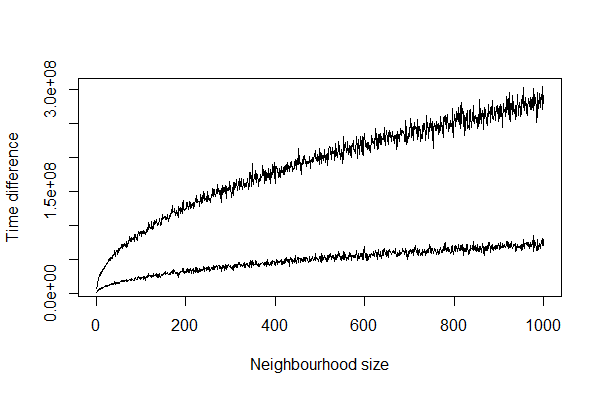
\includegraphics[width=0.9\linewidth]{ExperimentSimulat.png}
    \caption{Simulated Evolution of $T_g$ difference}
    \label{fig:experiment1b_simulated}
\end{figure}

When looking at Figure ~\ref*{fig:experiment1b_measured} and Figure ~\ref*{fig:experiment1b_simulated} we notice that increasing 
the neighborhood size of n produces a more noticeable gap between the "high" and "low" decryption times. In turn, this means that we can 
predict more accurately whether a bit of $q$ is 0 or 1. 

One significant difference between the two figures is that in the simulation the "low" time differences are also slightly increasing, probably due to the assumptions we previously made.
However, the general idea is still the same, as the gap between low and high values of $T_g$ increases indefinitely.

Some other experiments presented in the paper involve: testing the efficiency of the algorithm against randomly generated 1024-bit keys, analyzing the difference between inter-process and local network attacks, or testing the attack against different source-based optimizations.


\bibliography{mybib}
\bibliographystyle{plain}

\end{document}